\chapter{Discussion}

In the first chapter, we established that reading utilizes a variety of cognitive skills whose neural substrates are distributed throughout the brain. But being able to comprehend speech is a pre-requisite to reading, and it is similarly complex. This begs the question: in what ways is reading unique from listening?

The most widely-held view is that reading and listening share the same core linguistic processes and differ primarily in the sensory processes that feed into supra-model linguistic systems \citep{Mattingly1971, Price2012}. One popular model, the \textit{Simple View of Reading} states that reading comprehension is the product of listening comprehension and decoding skills \citep{Gough1986}. This view has received support from large behavioral studies \citep{Kirby2008} and neuroimaging investigations: many of the literacy-related changesare linked to visual or phonological systems, areas not directly related to semantic or comprehension processes \citep{Schlaggar2007, Dehaene2015}. These findings support a model in which inputs from auditory or visual domains are fed up into higher-order association areas that sequence, encode articulatory plans, and extract semantic information \citep{Price2012}. These processes localize onto the similar areas regardless of language and writing system \citep{Rueckl2016}, and may even extend to inputs from somatosensory domains \citep{Xu2005, Sood2016}. This supra-modal language core is largely left-lateralized and centers on the inferior frontal gyrus, anterior and posterior middle temporal gyrus and the angular gyrus. Neuroanatomical models of language, shown in Fig. \ref{ch3-price-language-models}, illustrate that language is distributed throughout much of the brain. 

\begin{figure}[t]
	\centering
	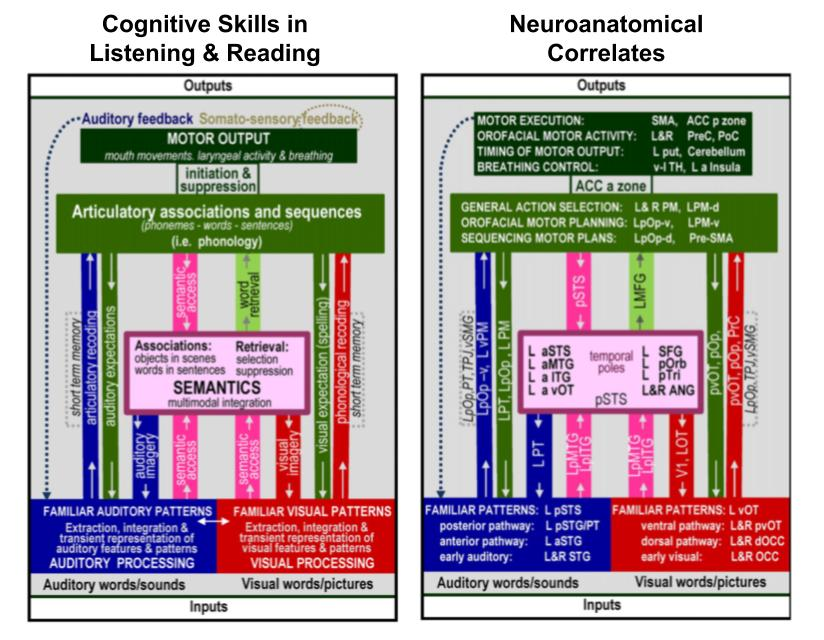
\includegraphics[height=3in]{images/ch3-price-language-models.jpg}
	\caption[Schematics of skills and brain areas used in reading.]{Models of reading typically focus on a common linguistic core that is responsible for comprehension and production of language. In this model, differences in modality affect input pathways to this core.}
	\label{fig:ch3-price-language-models}
\end{figure}

Despite the clear overlap between reading and listening, there is also evidence that the two skills are not directly equivalent. There is a subset of students who, despite adequate word decoding skills and vocabulary skills, struggle with reading comprehension\citep{Pimperton2010, Spencer2014}. From a neurobiological perspective, expected differences in primary visual (for reading) and primary auditory (for listening) represent the different input systems, with ventral occipito-temporal systems also activating \citep{Jobard2007}. However, differences in core language systems are also observed: additional activation in left posterior temporal and parietal areas in reading modality \citep{Constable2004}, as well increased bi-laterality especially in children \citep{Berl2011}. 

Most current cognitive models suggest that language comprehension requires the construction of a mental representation includes textual information and associated background knowledge, connected by some conscious and some unconscious executive processes \citep{Kendeou2014}. The parallel model shown in Fig. \ref{fig:ch3-price-language-models} is linear: it moves from sensation to action. During comprehension, however, the relationship between areas is dynamic and constantly being re-evaluated. The roles of attention and executive systems are likely to play an important role. Thus, while there may be a core set of systems for manipulating and extracting meaning from language, it is likely that differences in modality would modulate these processes. 

The pioneering researcher Alvin Liberman suggested that reading, instead of being parallel to listening, is actually parasitic: it requires an textit{awareness} of the linguistic act that is not required in listening. Brain activation studies may not capture these differences: it could very well be the interactions of different functional systems that are changed, rather than the overall ``engagement'' of an individual brain area. Additionally, the fact that reading integrates in an additinoal modality could be a source of difference, especially in emerging readers. 

In this study, we pursue three hypothesized ways reading might differ from listening. These are not exclusive; one or more of them may be true. The overarching aim is to test whether reading and listening differ only, or primarily, in their 

\begin{itemize}
	\item Reading will require a greater global reorganization of resting-state networks than listening. This network will also be more highly integrated than that of listening. 
	\item Reading will reduce the modularity within the sensory system of interest. That is, visual areas will become less internally connected during reading, while auditory areas will be less internally connected during listening.
	\item Reading will make greater demands on attention systems than listening. That is, areas in the frontal and attention systems will be activated to a greater degree during reading than listening.
\end{itemize}

%%%%

The current study sought to determine whether aspects of the brain's network architecture are related to reading. The results suggest that an efficient network organization, i.e. one in which brain areas form clusters connected by hub regions, is important for skilled reading, and that dyslexia can be characterized by abnormal functioning of hub regions that map information between multiple systems. To our knowledge, this is the first time the relationship between modularity and hubness to reading skill has been described, adding to a foundation of work built on other connectivity methods.

A connectomics approach to reading illuminates -- not displaces -- previous neuroimaging research, much of which focused on localizing specific cognitive processes. One insight is that much of the "reading network" falls in domain-general RSNs such as the attention and executive networks (see Fig. 1). While these areas perform a specific function in reading, they are also often involved in other processes. For example, the dorsal attention network (DAN) encompasses the visual word form area, an area that has been the subject of much interest and debate in reading and dyslexia research \citep{McCandliss2003}. It is probable that this area is so important in reading not only because it is connected to language areas \citep{Bouhali2014}, but also because it is tightly tied to other areas that control goal-directed attention \citep{Vogel2014}. Koyama et al. (2013) found that children with a historical diagnosis of dyslexia had persistent de-coupling of the DAN compared to typical readers regardless of remediation status \citep{Koyama2013}. Vogel et al. (2012) found that reading ability in typical children and adults (including decoding and passage comprehension ability) predicted increased correlations between the visual word form area and the DAN \citep{Vogel2012a}. The nesting of this orthographic-processing area within the DAN is thus important to its role in reading.

An efficient small-world organization in the resting brain requires a modular network architecture, which was tied here to better performance in reading. This relationship was particularly high in the visual, default mode, cingulo-opercular networks. It is not yet possible to say whether modularity within these specific RSNs correlates most highly with reading because of their functional roles in reading processes or whether they simply capture global trends better than other networks. There is some reason to suspect specificity, however. In studies of remediation-induced changes to connectivity, increased connectivity within the visual network \citep{Koyama2013} and cingulo-opercular network \citep{HorowitzKraus2015} have predicted reading improvement in dyslexic children. The default mode network, on the other hand, supports a wide range of cognitive processes important for comprehension, including theory of mind, narrative processing, and autobiographical recall \citep{Buckner2008, AbdulSabur2014}, and its cohesiveness during resting-state has been used to investigate other disorders \citep{Uddin2008}. Future work will need to examine not just the internal connectivity, but the relationships between these networks during reading and at rest. The default mode network, for example, is typically anti-correlated with "task-positive" networks such as the fronto-parietal network. A high degree of anti-correlation has been reported to be important for performance on a variety of cognitive processes \citep{Fox2005, Keller2015}, but recent work suggests that high modularity and connectivity of the default mode during higher-level cognition is fundamental to processes relying on self-referential and memory retrieval processes, such as those found in language \citep{Vatansever2015}. The dynamics behind these interactions will be important for further establishing a framwork for investigating the roles of specific networks during reading. 

The additional findings that hubs areas are key in dyslexia are not surprising: dyslexia has often been thought to be a disorder of combining information across different functional systems, and in the context of connectomics, hub areas play a privileged role in mediating information flow between RSN’s. For example, the posterior temporal sulcus connects visual and auditory networks by binding letters to sounds \citep{Blau2010, VanAtteveldt2009} and the inferior frontal gyrus has many different subdivisions supporting language parsing and manipulation \citep{Hagoort2005}. However, casting dyslexia dysfunction into a connectomics perspective opens up new hypotheses and research avenues. For example, the brain areas of interest and neuroimaging metrics can be unified across other developmental disorders, including ADHD, specific language impairment and autism \citep{Stam2014}. Another benefit is that it opens up many more avenues for investigating dyslexia using functional and diffusion MRI, which can be performed in younger children and without administering a cognitive task. 

\section{Dynamic modeling of network architecture}

We could use dynamic modeling....

\section{Individualized parcellations}

A caveat with connectomics analyses, including those presented here, are that results for the modularity analyses are often based on RSN parcellations from previous literature \citep{Power2011}. It is possible that in this sample of children, there were differences in network organization that resulted in a lower global modularity but were in fact due to differences in organization (e.g. multiple sub-modules of the default mode network). The question of how network architecture develops over time, and how best to measure it is under active investigation \citep{Cao2016}. Its answer will have important implications for disentangling this complex interchange between development, network architecture and cognitive performance.

